\subsubsection{\stid{4.14} VeloC: Very Low Overhead Checkpointing System} 

\paragraph{Overview} 

The VeloC-SZ project aims to provide VeloC, a high-performance, scalable
checkpoint/restart framework that leverages multi-level checkpointing
(the combination of several resilience strategies and heterogeneous
storage) to ensure that ECP applications run to completion with
minimal performance overhead. It delivers a production-ready solution
that increases development productivity by reducing the complexity of
having to deal with a heterogeneous storage stack and multiple vendor
APIs. VeloC offers a client library that can be used by the
applications to capture local application states, which are then
coordinated and persisted using a resilience engine.  VeloC runs the resilience engine asynchronously, which overlaps a large part of the checkpointing
with the application runtime, thereby reducing its overhead.

VeloC has been released and shows significant lower checkpointing
overhead for several ECP applications, such as HACC, LatticeQCD, 
EXAALT. VeloC is a next generation checkpointing system that builds on SCR, which won the prestigious R\&D 100 award in 2019. 

\paragraph{Key Challenges}
VeloC faces several key challenges:
\begin{itemize}
    \item \textbf{I/O bottlenecks:} applications typically employ simple checkpoint-restart mechanisms to survive failures that directly use a parallel file system. With diminishing I/O bandwidth available per 
    core, this leads to high checkpointing overhead and is not sustainable
    \item \textbf{Deep heterogeneous storage} To compensate for diminishing
    parallel file system I/O bandwidth per core, the storage stack
    is becoming increasingly deeper and heterogeneous: node-local NVRAM, burst buffers, key-value stores, etc. However, the variety of vendors and performance characteristics make it difficult for application developers to take advantage of it.
    \item \textbf{Restart-in-place:} a majority of failures affect only a small
    part of the nodes where the job is running. Therefore, reusing the 
    surviving nodes immediately after a failure is more efficient than
    submitting a new job (which may wait in the batch queue) that restarts from the latest checkpoint.
    \item \textbf{Portability and robustness:} applications need to run on
    a variety of supercomputing architectures, each featuring distinct
    capabilities. Their critical data structures that need to be checkpointed are constantly growing in size and complexity. Therefore,
    a flexible checkpointing solution is needed that can adapt to a variety
    of scenarios and configurations without sacrificing performance and scalability.
\end{itemize}

\paragraph{Solution Strategy}

To address these challenges, VeloC adopts the following principles:

\begin{itemize}
    \setlength{\itemindent}{-2em}
    \item \textbf{Multi-level checkpointing:} is based on the idea that
    a majority of failures can be mitigated without involving the parallel file system: node-local checkpoints can be used to recover from 
    software bugs, replication/erasure coding can be used to recover from 
    most combinations of node failures. This reduces the frequency of
    checkpointing to the parallel file system and therefore the I/O
    bottlenecks.
    \item \textbf{Asynchronous mode:} once a node-local checkpoint has been
    written, applications do not need to wait for replication, erasure
    coding or writes to the parallel file system: these can be applied
    in the background, while the application continues running. However,
    in this case, it is important to minimize interference.
    \item \textbf{Transparent use of heterogeneous storage:} we developed
    several techniques that can leverage a variety of 
    local storage (in-memory file systems, flash storage) and external
    storage (burst buffers, key-value stores, parallel file systems) options. These techniques select the best available storage options,
    tune them with the optimal parameters and leverage any vendor-specific
    API if needed to transfer data.
    \item \textbf{Job scheduler integration:} to implement restart-in-place,
    we have developed a series of scripts that interact with a variety
    of job schedulers to run jobs with spare nodes, continue execution on failures, restart on the surviving nodes and spares using the fastest possible recovery strategy (which ideally avoids reading checkpoints
    from the parallel file system). This is transparent to the users.
    \item \textbf{Declarative API and automated serialization:} 
    we offer a simple API that enables users to either manually
    capture checkpoints into files or to define memory regions
    that are automatically serialized into checkpoint files.
    \item \textbf{Modular design:} applications link with a client
    library that is responsible to manage local checkpoints, while
    a separate engine is responsible to employ the rest of the resilience
    strategies as plugin-able modules. This simplifies the implementation of the asynchronous mode, enables users the flexibility choose any
    combination of resilience strategies, as well as to customize 
    the checkpoiting pipeline (e.g., add new post-processing operations
    such as analytics or compression)
\end{itemize}
    
\paragraph{Recent Progress}

We met and closely collaborated with several ECP application teams in
an effort to address their checkpointing needs. Most of our current
efforts involve the HACC, LatticeQCD and EXAALT teams. The integration
with HACC aimed to isolate the checkpointing code in a plugin to enable
easier maintenance, ability to switch checkpointing on/off and sharing
of critical data used for checkpoints with other in-situ plugins (e.g., analytics, post-processing, etc.). To this end, we designed and 
implemented a VELOC checkpointing plugin for CosmoTools, the
in-situ framework used by HACC. For LatticeQCD and EXAALT, the integration
has been performed directly into the main code. Integration with 
other ECP applications is ongoing.

\begin{wrapfigure}{l}{0.47\textwidth}
  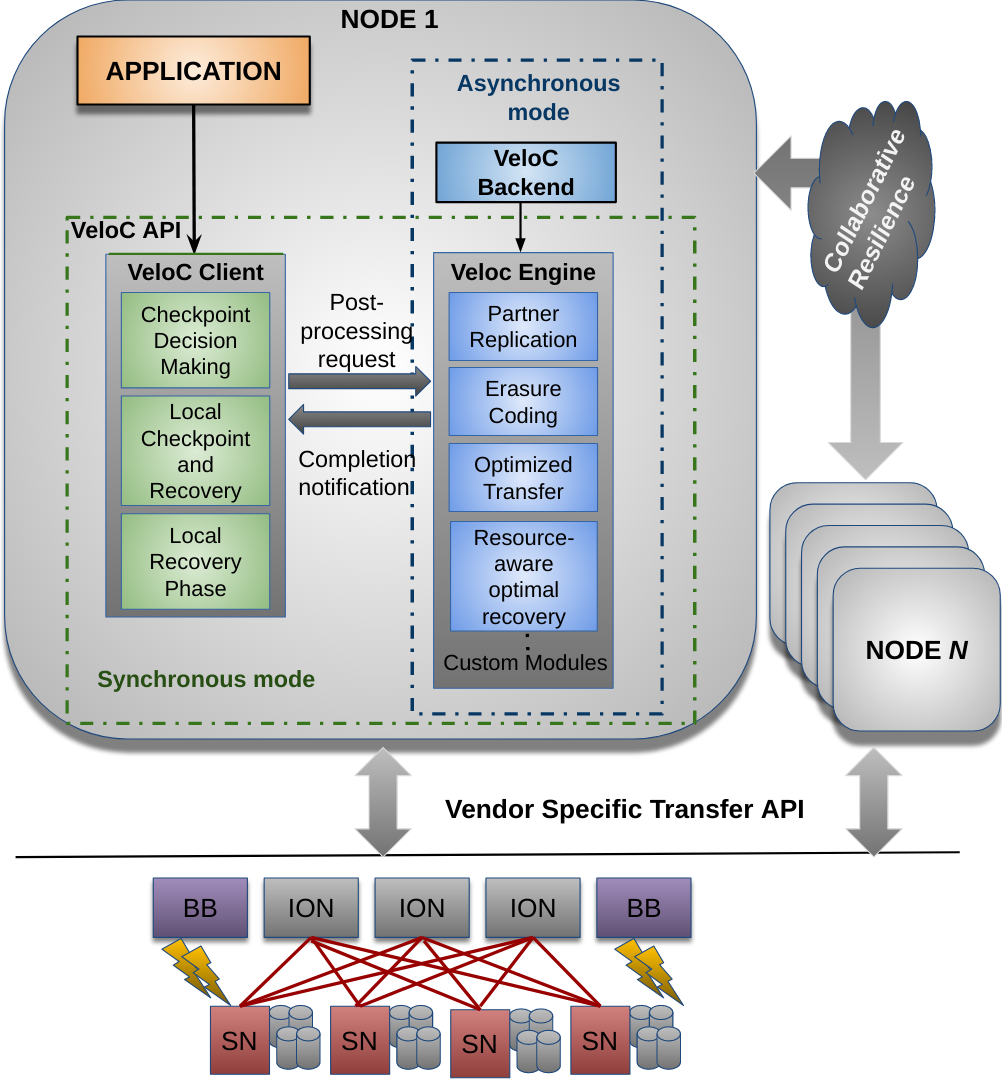
\includegraphics[width=0.4\textwidth]{projects/2.3.4-DataViz/2.3.4.14-VeloC-SZ/veloc-arch}
  \caption{VeloC: Architecture}%
  \label{fig:veloc:arch}%
\end{wrapfigure}


In parallel with the co-design effort done in collaboration with the
ECP application teams, we improved the asynchronous mode mentioned previously and illustrated in Figure~\ref{fig:veloc:arch}. Specifically, 
we have introduced an experimental hybrid local checkpointing strategy
that leverages hybrid local storage (memory, flash) simultaneously to
enable faster asynchronous flushes to the parallel file system~\cite{VeloCIPDPS19}. Furthermore, we have explored interference mitigation strategies
during asychronous checkpointing based on the prediction of shared
resource utilization, which can be used for better scheduling of
background operations~\cite{PredictionEuroPar19}.

The latest release v.1.2 introduces several new capabilities: (1) non-collective mode that enables processes
to checkpoint independently rather than as a single group;
(2) improved file-based mode that preserves custom file names
when flushing to the parallel file system, which is especially
useful for applications that make use of the SCR-to-VeloC 
compatibility translation library; (3) AXL, the library
responsible for transfers to/from external storage now auto-detects
and configures the best way to transfer files between local and
external storage.

In addition, we have added several new features that facilitate better integration with the ECP ecosystem: (1) restart-in-place scripts
for the following platforms: ANL Theta, ORNL Summit, LLNL Lassen;
(2) automated testing infrastructure based on Travis, which facilitates a smooth transition towards the ECP continuous integration initiative;
(3) Python bindings, which enables the use of VeloC in applications
that make use of high level analytics and artificial intelligence
libraries (e.g. Keras); (4) Spack installation packages and integration
into the OpenHPC distribution.

%\begin{figure}[t]
%  \begin{subfloat}[HACC\label{fig:veloc:hacc}]
%  \centering
%  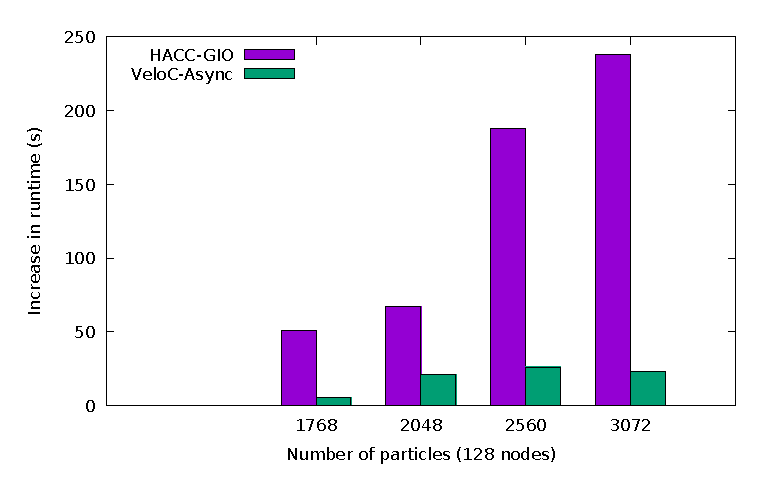
\includegraphics[width=.47\textwidth]{projects/2.3.4-DataViz/2.3.4.14-Vel%oC-SZ/veloc-hacc}
%  \end{subfloat}
%  \hfill
%  \begin{subfloat}[LatticeQCD\label{fig:veloc:lqcd}]
%  \centering
%  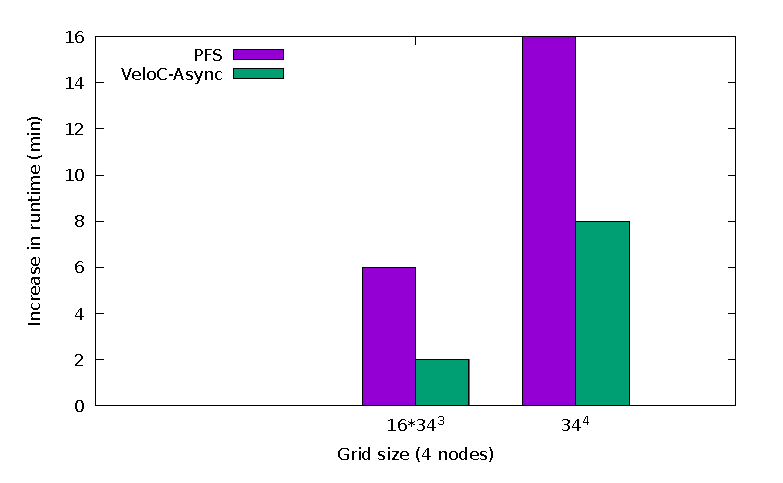
\includegraphics[width=.47\textwidth]{projects/2.3.4-DataViz/2.3.4.14-Vel%oC-SZ/veloc-lqcd}
%  \end{subfloat}
% \caption{VeloC results with ECP applications: increase in execution time %due to checkpointing (lower is better)}
%  \label{fig:veloc:results}%
%end{figure}

Finally we expanded the documentation and created tutorials that were
presented at various international venues to raise awareness about
VeloC within the broader HPC community at international level.

\paragraph{Next Steps}

We are working towards several goals: (1) improving the integration 
of VeloC  with resource managers to automate the process of checking 
the status of jobs and nodes, detect failures and relaunch jobs on failed nodes; (2) improving portability and robustness by introducing support for
flexible client-engine communication (e.g. Mercury) and advanced
serialization (e.g. C++ high-level data structures); (3) continue 
hardening the integration with existing ECP applications; (4) improve 
the automated testing infrastructure  and build environment for VeloC to support comprehensive testing on ECP machines. 

In parallel, we will continue to collaborate with the
application teams to address new requirements should they arise.
Furthermore, we will expand our user base beyond ECP to interact and
get feedback from the broader international community.
